\documentclass[11pt]{article}
\usepackage[margin=1in]{geometry}
\usepackage{amsmath,amssymb}
\usepackage{siunitx}
\usepackage{physics}
\usepackage{tikz}
\usetikzlibrary{arrows.meta,angles,quotes,calc,decorations.pathmorphing,decorations.markings}
\usepackage{enumitem}
\sisetup{per-mode=symbol}

\newcommand{\ans}[1]{\boxed{\displaystyle #1}}

\title{PHYS 121 --- HW4 Solutions}
\author{WRITTER}

\begin{document}
\maketitle
\setlist[itemize]{noitemsep,topsep=2pt}

% Helper constants
\def\g{\,\mathrm{g}}

\section*{Q1. A rotating grinding wheel (10 pts)}
Given: $M = \SI{50.0}{kg}$, diameter $D = \SI{1.0}{m}$, so radius $R = \SI{0.50}{m}$.

\textbf{(a) Spin-up torque:} From rest ($\omega_0 = 0$) to $\omega = \SI{120}{rev/min} = 4\pi~\text{rad/s} = \SI{12.6}{rad/s}$ in $\Delta\theta = 20$ revolutions $= 40\pi~\text{rad} = \SI{125.7}{rad}$.

Using rotational kinematics: $\omega^2 = \omega_0^2 + 2\alpha\Delta\theta$:
\[ \omega^2 = 2\alpha\Delta\theta \quad\Rightarrow\quad \alpha = \frac{\omega^2}{2\Delta\theta} = \frac{(4\pi)^2}{2 \times 40\pi} = \frac{16\pi^2}{80\pi} = \frac{\pi}{5} = \ans{\SI{0.628}{rad/s^2}}. \]

\textbf{Sketches:}
\begin{center}
\begin{tikzpicture}[scale=0.9]
  % ω-t plot
  \begin{scope}
    \draw[->,thick] (0,0) -- (5,0) node[right]{$t$};
    \draw[->,thick] (0,0) -- (0,3) node[above]{$\omega$};
    \draw[domain=0:4.5,smooth,variable=\x,thick,blue!80] plot (\x,{2.5*(\x/4.5)});
    \node[below] at (2.5,-0.5) {\textbf{$\omega$--$t$}};
    \node[right] at (4.5,2.5) {$\omega = \alpha t$};
  \end{scope}
  % θ-t plot
  \begin{scope}[xshift=6cm]
    \draw[->,thick] (0,0) -- (5,0) node[right]{$t$};
    \draw[->,thick] (0,0) -- (0,3) node[above]{$\theta$};
    \draw[domain=0:4.5,smooth,variable=\x,thick,blue!80] plot (\x,{2.5*(\x/4.5)^2});
    \node[below] at (2.5,-0.5) {\textbf{$\theta$--$t$}};
    \node[right] at (4.5,2.5) {$\theta = \frac{1}{2}\alpha t^2$};
  \end{scope}
\end{tikzpicture}
\end{center}

Moment of inertia for a cylinder: $I = \frac{1}{2}MR^2 = \frac{1}{2} \times 50.0 \times (0.50)^2 = \SI{6.25}{kg\cdot m^2}$.

Torque: $\tau = I\alpha = 6.25 \times 0.628 = \ans{\SI{3.93}{N\cdot m}}$.

\textbf{(b) Steady-speed torque:} Tool pressed perpendicularly at rim with $F = \SI{40.0}{N}$, $\mu_k = 0.60$.

\textbf{FBD at contact point:}
\begin{center}
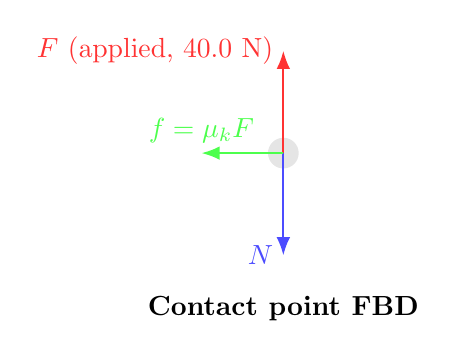
\begin{tikzpicture}[scale=1.3]
  % Contact point (blown up view)
  \coordinate (contact) at (0,0);
  \fill[gray!20] (contact) circle (0.15);
  % Applied force (perpendicular to rim)
  \draw[-{Latex},thick,red!80] (contact) -- (0,1) node[left]{$F$ (applied, 40.0 N)};
  % Normal force (equal and opposite to applied)
  \draw[-{Latex},thick,blue!70] (contact) -- (0,-1) node[left]{$N$};
  % Friction force (tangential, opposing rotation)
  \draw[-{Latex},thick,green!70] (contact) -- (-0.8,0) node[above]{$f = \mu_k F$};
  % Label
  \node[below] at (0,-1.3) {\textbf{Contact point FBD}};
\end{tikzpicture}
\end{center}

Friction force: $f = \mu_k F = 0.60 \times 40.0 = \SI{24.0}{N}$ (tangential, opposing rotation).

Friction torque (opposing rotation): $\tau_{\text{friction}} = fR = 24.0 \times 0.50 = \ans{\SI{12.0}{N\cdot m}}$.

To maintain constant $\omega$ (zero angular acceleration), the motor must provide equal and opposite torque: $\tau_{\text{motor}} = \tau_{\text{friction}} = \ans{\SI{12.0}{N\cdot m}}$.

\begin{center}
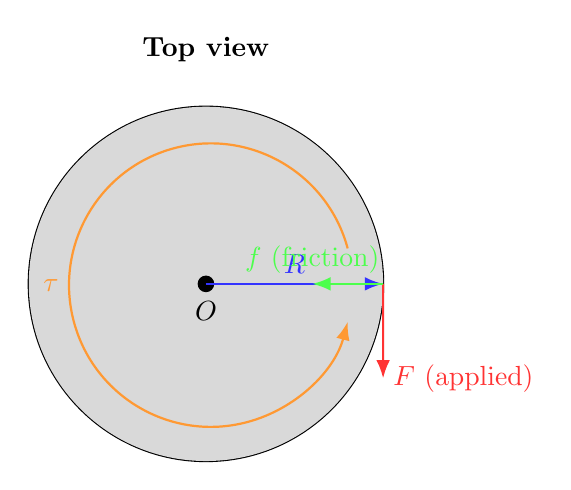
\begin{tikzpicture}[scale=1.5]
  % Top view of grinding wheel
  \draw[thick] (0,0) circle (1.5);
  \fill[gray!30] (0,0) circle (1.5);
  \fill (0,0) circle (2pt) node[below=3pt]{$O$};
  % Radius vector
  \draw[-{Latex},thick,blue!80] (0,0) -- (1.5,0) node[midway,above,sloped]{$R$};
  % Applied force at rim
  \coordinate (contact) at (1.5,0);
  \draw[-{Latex},thick,red!80] (contact) -- (1.5,-0.8) node[right]{$F$ (applied)};
  % Friction force
  \draw[-{Latex},thick,green!70] (contact) -- ++(-0.6,0) node[above]{$f$ (friction)};
  % Torque sense arrow (curved)
  \draw[-{Latex},thick,orange!80] (1.2,0.3) arc (15:345:1.2) node[left,midway]{$\tau$};
  % Label
  \node[above] at (0,1.8) {\textbf{Top view}};
\end{tikzpicture}
\end{center}

\section*{Q2. Two-groove Atwood pulley (10 pts)}
Given: Pulley with moment of inertia $I$, two radii $r_1$ and $r_2$ ($r_2 > r_1$), masses $m_1$ and $m_2$ ($m_2 > m_1$).

Choose positive rotation so that $m_2$ moves down (clockwise).

\textbf{(a) Angular acceleration:} Tensions $T_1$ and $T_2$ act on the pulley. For translation of masses:
\[ m_1 a_1 = T_1 - m_1 g, \quad m_2 a_2 = m_2 g - T_2. \]

No-slip condition: $a_1 = \alpha r_1$, $a_2 = \alpha r_2$.

Net torque on pulley: $\tau_{\text{net}} = T_2 r_2 - T_1 r_1 = I\alpha$.

Solving:
\begin{align*}
T_1 &= m_1(g + a_1) = m_1(g + \alpha r_1), \\
T_2 &= m_2(g - a_2) = m_2(g - \alpha r_2), \\
T_2 r_2 - T_1 r_1 &= I\alpha.
\end{align*}

Substituting:
\[ m_2(g - \alpha r_2)r_2 - m_1(g + \alpha r_1)r_1 = I\alpha. \]

\[ m_2 g r_2 - m_1 g r_1 - \alpha(m_2 r_2^2 + m_1 r_1^2) = I\alpha. \]

\[ m_2 g r_2 - m_1 g r_1 = \alpha(I + m_2 r_2^2 + m_1 r_1^2). \]

\[ \alpha = \ans{\frac{m_2 g r_2 - m_1 g r_1}{I + m_2 r_2^2 + m_1 r_1^2}}. \]

\textbf{(b) Linear accelerations:}
\[ a_1 = \alpha r_1 = \ans{\frac{(m_2 g r_2 - m_1 g r_1)r_1}{I + m_2 r_2^2 + m_1 r_1^2}} \quad \text{(upward)}, \]
\[ a_2 = \alpha r_2 = \ans{\frac{(m_2 g r_2 - m_1 g r_1)r_2}{I + m_2 r_2^2 + m_1 r_1^2}} \quad \text{(downward)}. \]

\begin{center}
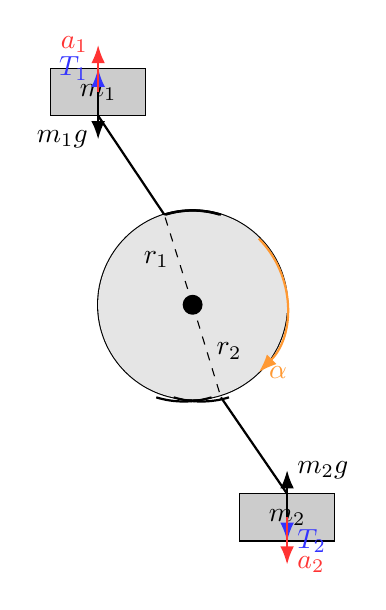
\begin{tikzpicture}[scale=1.2]
  % Pulley
  \draw[thick] (0,0) circle (1);
  \fill[gray!20] (0,0) circle (1);
  % Two grooves
  \draw[thick] (-0.3,0.954) arc (107:73:1);
  \draw[thick] (0.3,0.954) arc (73:107:1);
  \draw[thick] (-0.2,-0.980) arc (-107:-73:1);
  \draw[thick] (0.2,-0.980) arc (-73:-107:1);
  % Axle
  \fill (0,0) circle (3pt);
  % Masses
  \draw[fill=gray!40] (-1.5,2) rectangle (-0.5,2.5) node[midway]{$m_1$};
  \draw[fill=gray!40] (0.5,-2.5) rectangle (1.5,-2) node[midway]{$m_2$};
  % Strings
  \draw[thick] (-1,2) -- (-0.3,0.954);
  \draw[thick] (1,-2) -- (0.3,-0.980);
  % Tensions
  \draw[-{Latex},thick,blue!80] (-1,2) -- (-1,2.5) node[left]{$T_1$};
  \draw[-{Latex},thick,blue!80] (1,-2) -- (1,-2.5) node[right]{$T_2$};
  % Accelerations
  \draw[-{Latex},thick,red!80] (-1,2.25) -- (-1,2.75) node[left]{$a_1$};
  \draw[-{Latex},thick,red!80] (1,-2.25) -- (1,-2.75) node[right]{$a_2$};
  % Radii
  \draw[dashed] (0,0) -- (-0.3,0.954) node[midway,left]{$r_1$};
  \draw[dashed] (0,0) -- (0.3,-0.980) node[midway,right]{$r_2$};
  % Rotation arrow
  \draw[-{Latex},thick,orange!80] (0.7,0.7) arc (45:-45:1) node[right]{$\alpha$};
  % Gravity
  \draw[-{Latex},thick] (-1,2.25) -- (-1,1.75) node[left]{$m_1g$};
  \draw[-{Latex},thick] (1,-2.25) -- (1,-1.75) node[right]{$m_2g$};
\end{tikzpicture}
\end{center}

\section*{Q3. Rotating stick with end masses (10 pts)}
Given: Stick length $L = \SI{1.0}{m}$, mass $M = \SI{6.0}{kg}$, pivots about center. Masses $m_1 = \SI{4.0}{kg}$ and $m_2 = \SI{2.5}{kg}$ at ends. Released from horizontal.

\textbf{(a) Drawing:}
\begin{center}
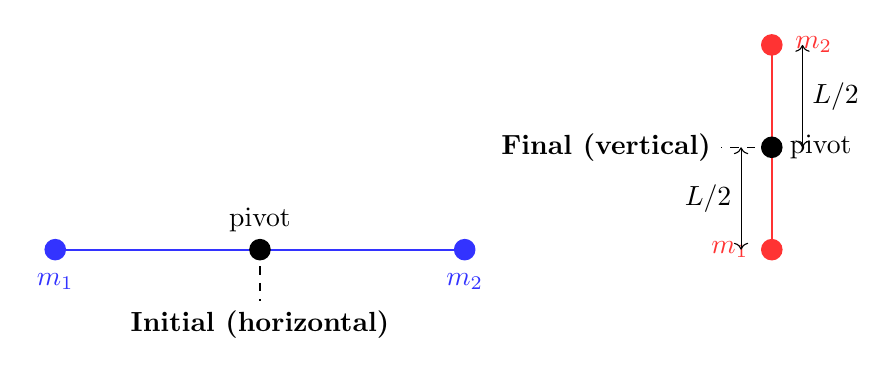
\begin{tikzpicture}[scale=1.3]
  % Initial position (horizontal)
  \draw[thick,blue!80] (-2,0) -- (2,0);
  \fill[blue!80] (-2,0) circle (3pt) node[below=5pt]{$m_1$};
  \fill[blue!80] (2,0) circle (3pt) node[below=5pt]{$m_2$};
  \fill (0,0) circle (3pt) node[above=3pt]{pivot};
  \draw[dashed] (0,0) -- (0,-0.5) node[below]{\textbf{Initial (horizontal)}};
  % Final position (vertical)
  \begin{scope}[xshift=5cm]
    \draw[thick,red!80] (0,0) -- (0,2);
    \fill[red!80] (0,0) circle (3pt) node[left=5pt]{$m_1$};
    \fill[red!80] (0,2) circle (3pt) node[right=5pt]{$m_2$};
    \fill (0,1) circle (3pt) node[right=3pt]{pivot};
    \draw[dashed] (0,1) -- (-0.5,1) node[left]{\textbf{Final (vertical)}};
    % Height markers
    \draw[<->] (-0.3,0) -- (-0.3,1) node[midway,left]{$L/2$};
    \draw[<->] (0.3,1) -- (0.3,2) node[midway,right]{$L/2$};
  \end{scope}
\end{tikzpicture}
\end{center}

\textbf{(b) Energy method:} Only the end masses change gravitational energy. The stick's center of mass remains at the pivot, so $\Delta U_{\text{stick}} = 0$.

Initial: Both masses at height $h_0 = 0$ (taking pivot as reference).

Final: $m_1$ at height $-L/2 = -\SI{0.50}{m}$, $m_2$ at height $L/2 = \SI{0.50}{m}$.

\[ \Delta U = m_1 g(-L/2) + m_2 g(L/2) = g(m_2 - m_1)L/2 = 9.8 \times (2.5 - 4.0) \times 0.50 = \ans{\SI{-7.35}{J}}. \]

The negative sign indicates energy is released (converted to kinetic energy).

\textbf{(c) Rotational inertia and angular speed:} Rotational inertia about the pivot:
\[ I = I_{\text{stick}} + m_1(L/2)^2 + m_2(L/2)^2. \]

For a stick pivoted at center: $I_{\text{stick}} = \frac{1}{12}ML^2$.

\[ I = \frac{1}{12} \times 6.0 \times 1.0^2 + 4.0 \times 0.50^2 + 2.5 \times 0.50^2 = 0.50 + 1.00 + 0.625 = \SI{2.125}{kg\cdot m^2}. \]

Conservation of energy: $\Delta K + \Delta U = 0$, so $K_{\text{final}} = -\Delta U = \SI{7.35}{J}$.

\[ \frac{1}{2}I\omega^2 = 7.35 \quad\Rightarrow\quad \omega = \sqrt{\frac{2 \times 7.35}{2.125}} = \sqrt{6.918} = \ans{\SI{2.63}{rad/s}}. \]

\textbf{(d) Checks:}
\begin{itemize}
  \item If $m_1 = m_2$: $\Delta U = g(m_2 - m_1)L/2 = 0$, so $\omega = 0$ (no rotation, balanced).
  \item If $m_2 \to 0$: Only $m_1$ at distance $L/2$ from pivot. $I = \frac{1}{12}ML^2 + m_1(L/2)^2$, $\Delta U = -m_1 g L/2$, giving $\omega = \sqrt{m_1 g L / I}$. This matches a single point mass at $L/2$ if the stick is massless ($M = 0$), in which case $I = m_1(L/2)^2$ and $\omega = \sqrt{2g/L}$.
\end{itemize}

\section*{Q4. Spring-pushed sphere that skids then rolls (17 pts)}
Given: Solid ball mass $m$, radius $r$, spring constant $k$, compression $x$. Initially at rest on level surface.

\textbf{(a) Initial translational velocity:} Energy stored in spring: $U_{\text{spring}} = \frac{1}{2}kx^2$.

Assuming ball is not rotating and no friction, all energy goes to translational kinetic energy:
\[ \frac{1}{2}mv_i^2 = \frac{1}{2}kx^2 \quad\Rightarrow\quad v_i = \ans{\sqrt{\frac{kx^2}{m}} = x\sqrt{\frac{k}{m}}}. \]

\textbf{(b) Angular momentum about contact point:} Initially, ball is not rotating, so angular momentum about contact point is:
\[ L = mv_i r = \ans{mr x\sqrt{\frac{k}{m}} = xr\sqrt{km}}. \]

\textbf{(c) Moment of inertia about contact point:} Using parallel axis theorem. For a solid sphere about its center: $I_{\text{cm}} = \frac{2}{5}mr^2$.

About the contact point: $I = I_{\text{cm}} + mr^2 = \frac{2}{5}mr^2 + mr^2 = \ans{\frac{7}{5}mr^2}$.

\textbf{(d) Final velocity from angular momentum conservation:} When rolling without slipping, $v_f = \omega r$, so $\omega = v_f/r$.

Angular momentum about contact point (conserved): $L = I\omega = \frac{7}{5}mr^2 \cdot \frac{v_f}{r} = \frac{7}{5}mrv_f$.

Conservation: $mv_i r = \frac{7}{5}mrv_f$, so $v_f = \frac{5}{7}v_i = \ans{\frac{5}{7}x\sqrt{\frac{k}{m}}}$.

\textbf{(e) Energy dissipated:} Initial energy: $E_i = \frac{1}{2}kx^2$.

Final energy (rolling): $E_f = \frac{1}{2}mv_f^2 + \frac{1}{2}I_{\text{cm}}\omega^2 = \frac{1}{2}mv_f^2 + \frac{1}{2} \cdot \frac{2}{5}mr^2 \cdot \frac{v_f^2}{r^2} = \frac{1}{2}mv_f^2 + \frac{1}{5}mv_f^2 = \frac{7}{10}mv_f^2$.

Using $v_f = \frac{5}{7}v_i$ and $v_i^2 = \frac{kx^2}{m}$:
\[ E_f = \frac{7}{10}m \cdot \frac{25}{49}v_i^2 = \frac{7}{10} \cdot \frac{25}{49} \cdot kx^2 = \frac{5}{14}kx^2. \]

Energy dissipated: $\Delta E = E_i - E_f = \frac{1}{2}kx^2 - \frac{5}{14}kx^2 = \frac{7-5}{14}kx^2 = \frac{2}{14}kx^2 = \frac{1}{7}kx^2$.

Percentage: $\frac{\Delta E}{E_i} \times 100\% = \frac{1/7}{1/2} \times 100\% = \frac{2}{7} \times 100\% = \ans{\SI{28.6}{\percent}}$.

\textbf{(f) Toy estimate:} $F = \SI{10}{N}$ to compress $x = \SI{1}{cm} = \SI{0.01}{m}$, so $k = F/x = \SI{1000}{N/m}$.

Ball size of grape: mass $m \approx \SI{5}{g} = \SI{0.005}{kg}$, radius $r \approx \SI{1}{cm} = \SI{0.01}{m}$.

\[ v_f = \frac{5}{7} \times 0.01 \times \sqrt{\frac{1000}{0.005}} = \frac{5}{7} \times 0.01 \times \sqrt{200000} = \frac{5}{7} \times 0.01 \times 447.2 = \ans{\SI{3.19}{m/s}}. \]

\section*{Q5. Paper roll on an accelerating truck (10 pts)}
Given: Solid cylindrical roll on flat truck bed. Truck accelerates forward at constant $a$.

\textbf{1) Newton's 2nd law:} In ground frame, for translation:
\[ ma_{\text{cm}} = f, \]
where $f$ is the friction force (forward, driving the roll).

For rotation about center of mass:
\[ I\alpha = fR, \]
where $I = \frac{1}{2}mR^2$ for solid cylinder, and $f$ provides torque.

\textbf{2) No-slip condition:} Acceleration of contact point equals truck's acceleration:
\[ a_{\text{contact}} = a_{\text{cm}} + R\alpha = a. \]

From rotational equation: $\alpha = \frac{fR}{I} = \frac{fR}{mR^2/2} = \frac{2f}{mR}$.

Substituting: $a_{\text{cm}} + R \cdot \frac{2f}{mR} = a_{\text{cm}} + \frac{2f}{m} = a$.

From translational equation: $f = ma_{\text{cm}}$, so:
\[ a_{\text{cm}} + \frac{2ma_{\text{cm}}}{m} = 3a_{\text{cm}} = a \quad\Rightarrow\quad a_{\text{cm}} = \ans{\frac{a}{3}}. \]

\textbf{3) Relative acceleration:} The roll's acceleration relative to the truck:
\[ a_{\text{rel}} = a_{\text{cm}} - a = \frac{a}{3} - a = \ans{-\frac{2a}{3}}. \]

Negative sign indicates the roll accelerates backward relative to the truck.

\textbf{4) Distance to drop:} If the roll starts at the front edge and the truck bed has length $L$, the roll reaches the back edge when:
\[ s_{\text{truck}} = \frac{1}{2}at^2, \quad s_{\text{roll}} = \frac{1}{2}a_{\text{cm}}t^2 = \frac{1}{2} \cdot \frac{a}{3}t^2 = \frac{at^2}{6}. \]

Relative distance: $s_{\text{rel}} = s_{\text{truck}} - s_{\text{roll}} = \frac{at^2}{2} - \frac{at^2}{6} = \frac{at^2}{3}$.

For the roll to reach the back (relative distance = $L$):
\[ L = \frac{at^2}{3} \quad\Rightarrow\quad t^2 = \frac{3L}{a}. \]

Distance truck moves: $s = \frac{1}{2}at^2 = \frac{1}{2}a \cdot \frac{3L}{a} = \ans{\frac{3L}{2}}$.

\section*{Q6. Bug hits a hanging stick (10 pts)}
Given: Bug (mass $m_b$, speed $u$) hits and sticks to end of uniform stick (length $L$, mass $M = 10m_b$), pivoted at top, hanging vertically.

\textbf{1) Angular momentum conservation:} About the pivot, before impact: bug has angular momentum $L_i = m_b u L$ (perpendicular distance is $L$).

After impact: stick + bug rotate with angular speed $\omega$. Rotational inertia about pivot:
\[ I = I_{\text{stick}} + m_b L^2 = \frac{1}{3}ML^2 + m_b L^2 = \frac{1}{3} \cdot 10m_b L^2 + m_b L^2 = \frac{10m_b L^2}{3} + m_b L^2 = \frac{13m_b L^2}{3}. \]

Conservation: $m_b u L = I\omega = \frac{13m_b L^2}{3}\omega$.

\[ \omega = \frac{3m_b u L}{13m_b L^2} = \ans{\frac{3u}{13L}}. \]

\textbf{2) Maximum angle:} After impact, energy is conserved. Initial kinetic energy:
\[ K_i = \frac{1}{2}I\omega^2 = \frac{1}{2} \cdot \frac{13m_b L^2}{3} \cdot \left(\frac{3u}{13L}\right)^2 = \frac{13m_b L^2}{6} \cdot \frac{9u^2}{169L^2} = \frac{3m_b u^2}{26}. \]

At maximum angle $\theta$, the center of mass rises. The stick's center of mass is at $L/2$ from pivot, bug is at $L$ from pivot.

Initial center of mass distance from pivot: $d_{\text{cm}} = \frac{M \cdot L/2 + m_b \cdot L}{M + m_b} = \frac{10m_b \cdot L/2 + m_b L}{11m_b} = \frac{6m_b L}{11m_b} = \frac{6L}{11}$.

Taking the pivot as the reference (height $h = 0$), initially the center of mass is at height $h_i = -\frac{6L}{11}$ (below the pivot).

At maximum angle $\theta$ from vertical, the center of mass is at height $h_f = -\frac{6L}{11}\cos\theta$.

Rise: $\Delta h = h_f - h_i = -\frac{6L}{11}\cos\theta - \left(-\frac{6L}{11}\right) = \frac{6L}{11}(1 - \cos\theta)$.

Energy conservation: $K_i = (M + m_b)g\Delta h = 11m_b g \cdot \frac{6L}{11}(1 - \cos\theta) = 6m_b g L(1 - \cos\theta)$.

\[ \frac{3m_b u^2}{26} = 6m_b g L(1 - \cos\theta) \quad\Rightarrow\quad 1 - \cos\theta = \frac{u^2}{52gL}. \]

\[ \cos\theta = 1 - \frac{u^2}{52gL}. \]

Solving for $L$:
\[ \frac{u^2}{52gL} = 1 - \cos\theta \quad\Rightarrow\quad L = \ans{\frac{u^2}{52g(1 - \cos\theta)}}. \]

\textbf{3) Check:} If $\theta \to 0$, then $1 - \cos\theta \to 0$, so $L \to \infty$. This makes sense: to achieve only a tiny swing, the stick must be very long (small angular speed, large moment of inertia).

\section*{Q7. Ice-skating twirl and the double Axel (15 pts)}
Given: Skater as solid cylinder: height $h = \SI{1.50}{m}$, radius $R = \SI{10.0}{cm} = \SI{0.10}{m}$, mass $M = \SI{45}{kg}$. Two arms: each length $\ell = \SI{0.60}{m}$, mass $m_a = \SI{2.4}{kg}$. Arms can be extended or against cylinder.

\textbf{(a) Rotational inertia:}

\textbf{i) Arms at side:} Arms treated as thin rods against cylinder surface. For a thin rod of length $\ell$ and mass $m$ about one end: $I = \frac{1}{3}m\ell^2$. But if held against cylinder, they contribute as point masses at distance $R$ from axis: $I_{\text{arms}} = 2 \times m_a R^2 = 2 \times 2.4 \times 0.10^2 = \SI{0.048}{kg\cdot m^2}$.

Actually, if arms are against the cylinder, their center of mass is at $R$ from axis, so: $I_{\text{arms}} = 2 \times m_a R^2 = \SI{0.048}{kg\cdot m^2}$.

Cylinder: $I_{\text{cylinder}} = \frac{1}{2}MR^2 = \frac{1}{2} \times 45 \times 0.10^2 = \SI{0.225}{kg\cdot m^2}$.

Total: $I_1 = 0.225 + 0.048 = \ans{\SI{0.273}{kg\cdot m^2}}$.

\textbf{ii) Arms extended:} Each arm extends perpendicular from the cylinder surface. If the arm is a thin rod of length $\ell$ with its inner end at distance $R$ from the axis, the center of mass is at distance $R + \ell/2 = 0.10 + 0.30 = \SI{0.40}{m}$ from the axis.

Using parallel axis theorem: $I_{\text{arm}} = I_{\text{cm}} + m_a d^2$, where $I_{\text{cm}} = \frac{1}{12}m_a\ell^2$ (rod about its center) and $d = R + \ell/2 = \SI{0.40}{m}$.

\[ I_{\text{arm}} = \frac{1}{12}m_a\ell^2 + m_a(R + \ell/2)^2 = \frac{1}{12} \times 2.4 \times 0.60^2 + 2.4 \times 0.40^2 = 0.072 + 0.384 = \SI{0.456}{kg\cdot m^2}. \]

For two arms: $I_{\text{arms}} = 2 \times 0.456 = \SI{0.912}{kg\cdot m^2}$.

Total: $I_2 = 0.225 + 0.912 = \ans{\SI{1.137}{kg\cdot m^2}}$.

\textbf{(b) Time in air:} Maximum height $h_{\text{max}} = \SI{0.9}{m}$. Using $v^2 = v_0^2 - 2gh$, at maximum height $v = 0$:
\[ 0 = v_0^2 - 2gh_{\text{max}} \quad\Rightarrow\quad v_0 = \sqrt{2gh_{\text{max}}} = \sqrt{2 \times 9.8 \times 0.9} = \sqrt{17.64} = \SI{4.2}{m/s}. \]

Time to reach maximum: $t_{\text{up}} = v_0/g = 4.2/9.8 = \SI{0.429}{s}$.

Total time in air: $T = 2t_{\text{up}} = \ans{\SI{0.86}{s}}$.

\textbf{(c) Necessary rotational speed:} For 2.5 rotations in time $T = \SI{0.86}{s}$:
\[ \theta = 2.5 \times 2\pi = 5\pi \text{ rad}. \]

\[ \omega = \frac{\theta}{T} = \frac{5\pi}{0.86} = \ans{\SI{18.3}{rad/s} = \SI{175}{rev/min}}. \]

\textbf{(d) Configuration and initial speed:} To achieve high $\omega$, start with arms extended (larger $I$) and small $\omega_i$, then pull arms in (smaller $I$) to increase $\omega$ via angular momentum conservation.

Angular momentum conservation: $I_2 \omega_i = I_1 \omega_f$, where $\omega_f = \SI{18.3}{rad/s}$.

\[ \omega_i = \frac{I_1}{I_2} \omega_f = \frac{0.273}{1.137} \times 18.3 = 0.240 \times 18.3 = \ans{\SI{4.39}{rad/s}}. \]

So: start with arms extended, $\omega_i = \SI{4.39}{rad/s}$, then quickly pull arms in to achieve $\omega_f = \SI{18.3}{rad/s}$.

\textbf{(e) Landing with one leg extended:} Extending one leg increases moment of inertia, which decreases angular speed via conservation of angular momentum. This allows better control and stability upon landing, preventing over-rotation.

\section*{Q8. Three-force balance on a massless rod (10 pts)}
Given: Massless rod with three perpendicular forces at points A, B, C. Rod in static equilibrium. From the figure: point A is at \SI{0.3}{m} from left end, point B at \SI{0.7}{m} from left end, point C at \SI{10.4}{m} from left end. Force $F_C = \SI{100}{N}$ downward at point C.

For static equilibrium: $\sum \vec{F} = 0$ and $\sum \tau = 0$ (about any point).

Taking upward as positive, force balance:
\[ F_A + F_B + F_C = 0 \quad\Rightarrow\quad F_A + F_B - 100 = 0 \quad\Rightarrow\quad F_A + F_B = \SI{100}{N}. \]

Taking torques about point A (where $F_A$ acts, so its torque is zero). Distances: $d_{AB} = 0.7 - 0.3 = \SI{0.4}{m}$, $d_{AC} = 10.4 - 0.3 = \SI{10.1}{m}$.

Torque balance about A (taking counterclockwise as positive). Since $F_C$ is downward and acts to the right of A, it creates a clockwise (negative) torque. $F_B$ must create a counterclockwise (positive) torque, so it must be upward:
\[ F_B \cdot d_{AB} - F_C \cdot d_{AC} = 0. \]

With $F_C = \SI{100}{N}$ (downward, magnitude) and distances in meters:
\[ F_B \times 0.4 - 100 \times 10.1 = 0 \quad\Rightarrow\quad 0.4F_B = 1010 \quad\Rightarrow\quad F_B = \frac{1010}{0.4} = \ans{\SI{2525}{N}} \quad \text{(upward)}. \]

From force balance (taking upward as positive): $F_A + F_B + F_C = 0$, so $F_A + 2525 - 100 = 0$, giving:
\[ F_A = 100 - 2525 = \ans{\SI{-2425}{N}} = \SI{2425}{N} \text{ downward}. \]

\textbf{Verification:} Taking torques about point B (taking counterclockwise as positive):
- $F_A$ (downward, left of B): creates clockwise torque = $-|F_A| \times d_{AB} = -2425 \times 0.4 = -970$ N·m
- $F_C$ (downward, right of B): creates counterclockwise torque = $+|F_C| \times d_{BC} = 100 \times 9.7 = 970$ N·m
- Net torque: $-970 + 970 = 0$ (verified).

Taking torques about point C (taking counterclockwise as positive):
- $F_A$ (downward, left of C): creates counterclockwise torque = $-F_A \times d_{AC} = -(-2425) \times 10.1 = 24492.5$ N·m
- $F_B$ (upward, left of C): creates clockwise torque = $-F_B \times d_{BC} = -2525 \times 9.7 = -24492.5$ N·m
- Net torque: $24492.5 - 24492.5 = 0$ (verified).

\textbf{Summary:}
\begin{itemize}
  \item $F_A = \ans{\SI{2425}{N}}$ downward
  \item $F_B = \ans{\SI{2525}{N}}$ upward  
  \item $F_C = \SI{100}{N}$ downward (given)
\end{itemize}

\section*{Q9. Spider silk realism + Spiderman (16 pts)}
Given: Elastic modulus $Y = \SI{25}{GPa} = \SI{2.5e10}{N/m^2}$. For silk thread: length $L$, cross-sectional area $A$, stretch $x$, tension $F = YA x/L$.

Spider: mass $m = \SI{50}{mg} = \SI{5e-5}{kg}$, line diameter $d = \SI{0.14}{mm} = \SI{1.4e-4}{m}$, length $L = \SI{50}{cm} = \SI{0.50}{m}$.

\textbf{(a) Stretch:} Cross-sectional area: $A = \pi(d/2)^2 = \pi \times (7 \times 10^{-5})^2 = \pi \times 4.9 \times 10^{-9} = \SI{1.54e-8}{m^2}$.

Tension equals weight: $F = mg = 5 \times 10^{-5} \times 9.8 = \SI{4.9e-4}{N}$.

\[ F = \frac{YA x}{L} \quad\Rightarrow\quad x = \frac{FL}{YA}. \]

\[ x = \frac{4.9 \times 10^{-4} \times 0.50}{2.5 \times 10^{10} \times 1.54 \times 10^{-8}} = \frac{2.45 \times 10^{-4}}{3.85 \times 10^{2}} = \ans{\SI{6.36e-7}{m} = \SI{0.636}{\micro\meter}}. \]

\textbf{(b) Potential energy:} $U = \frac{1}{2}kx^2$, where effective spring constant $k = YA/L$.

\[ k = \frac{2.5 \times 10^{10} \times 1.54 \times 10^{-8}}{0.50} = \SI{7.7e2}{N/m}. \]

\[ U = \frac{1}{2} \times 770 \times (6.36 \times 10^{-7})^2 = \frac{1}{2} \times 770 \times 4.04 \times 10^{-13} = \ans{\SI{1.56e-10}{J}}. \]

\textbf{(c) Speed:} If all energy converts to kinetic: $\frac{1}{2}mv^2 = U$.

\[ v = \sqrt{\frac{2U}{m}} = \sqrt{\frac{2 \times 1.56 \times 10^{-10}}{5 \times 10^{-5}}} = \sqrt{6.24 \times 10^{-6}} = \ans{\SI{2.50e-3}{m/s} = \SI{2.50}{mm/s}}. \]

\textbf{(d) Drawing:}
\begin{center}
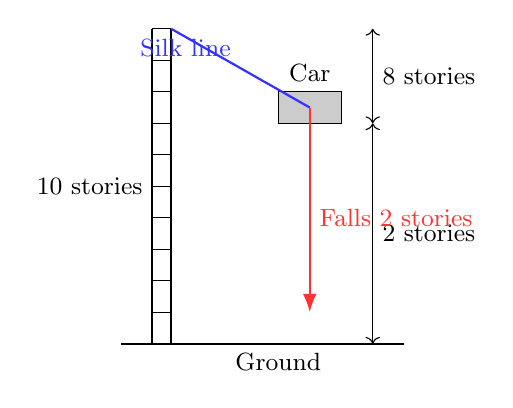
\begin{tikzpicture}[scale=0.8]
  % Parking garage (10 stories)
  \draw[thick] (0,0) -- (0,5);
  \draw[thick] (0.3,0) -- (0.3,5);
  \foreach \y in {0.5,1,1.5,2,2.5,3,3.5,4,4.5,5} {
    \draw (0,\y) -- (0.3,\y);
  }
  \node[left] at (0,2.5) {\small 10 stories};
  % Car falling
  \draw[fill=gray!40] (2,3.5) rectangle (3,4);
  \node[above] at (2.5,4) {\small Car};
  % Silk line
  \draw[thick,blue!80] (0.3,5) -- (2.5,3.75);
  \node[above left,blue!80] at (1.4,4.4) {\small Silk line};
  % Ground
  \draw[thick] (-0.5,0) -- (4,0);
  \node[below] at (2,0) {\small Ground};
  % Height markers
  \draw[<->] (3.5,0) -- (3.5,3.5) node[midway,right] {\small 2 stories};
  \draw[<->] (3.5,3.5) -- (3.5,5) node[midway,right] {\small 8 stories};
  % Arrow showing fall
  \draw[-{Latex},thick,red!80] (2.5,3.75) -- (2.5,0.5);
  \node[right,red!80] at (2.5,2) {\small Falls 2 stories};
\end{tikzpicture}
\end{center}

\textbf{(e) Minimum diameter (infinitely elastic):} Car falls 2 stories. Assume story height $\approx \SI{3}{m}$, so fall height from connection point to ground $h = \SI{6}{m}$. Car mass $m_{\text{car}} \approx \SI{1500}{kg}$.

Car falls from top (10 stories) and line connects at 2 stories above ground. Distance fallen: $h = 8 \times \SI{3}{m} = \SI{24}{m}$. Speed at connection: $v = \sqrt{2gh} = \sqrt{2 \times 9.8 \times 24} = \sqrt{470.4} = \SI{21.7}{m/s}$.

Car must stop at ground (additional 2 stories = $\SI{6}{m}$). Kinetic energy to absorb: $K = \frac{1}{2}mv^2 = \frac{1}{2} \times 1500 \times (21.7)^2 = \SI{3.53e5}{J}$.

If the line is infinitely elastic and stretches by $x = \SI{6}{m}$ (the distance car falls after connection), the energy stored is $U = \frac{1}{2}kx^2$, where $k = YA/L_0$.

Assuming the line's unstretched length is approximately the connection height ($L_0 \approx \SI{6}{m}$), then:
\[ U = \frac{1}{2} \cdot \frac{YA}{L_0} \cdot x^2 = \frac{1}{2} \cdot \frac{YA}{6} \cdot 36 = 3YA. \]

Setting $U = K = \SI{3.53e5}{J}$:
\[ 3 \times 2.5 \times 10^{10} \times A = 3.53 \times 10^5 \quad\Rightarrow\quad A = \frac{3.53 \times 10^5}{7.5 \times 10^{10}} = \SI{4.71e-6}{m^2}. \]

\[ d = 2\sqrt{\frac{A}{\pi}} = 2\sqrt{\frac{4.71 \times 10^{-6}}{\pi}} = 2\sqrt{1.50 \times 10^{-6}} = 2 \times 1.225 \times 10^{-3} = \ans{\SI{2.45e-3}{m} = \SI{2.45}{mm}}. \]

\textbf{(f) Would the line break?} Real silk has a breaking stress. Typical spider silk breaking stress $\sigma_{\text{max}} \approx \SI{1}{GPa} = \SI{1e9}{Pa}$ (dragline silk can be higher, up to $\sim\SI{1.3}{GPa}$, but we'll use $\SI{1}{GPa}$).

Maximum tension: $F_{\text{max}} = \sigma_{\text{max}} A = 1 \times 10^9 \times 4.71 \times 10^{-6} = \SI{4.71e3}{N} = \SI{4710}{N}$.

The tension in the line when stretched by $x$ is $F = kx = \frac{YA}{L_0}x$. For $x = \SI{6}{m}$ and $L_0 = \SI{6}{m}$:
\[ F = \frac{2.5 \times 10^{10} \times 4.71 \times 10^{-6}}{6} \times 6 = 2.5 \times 10^{10} \times 4.71 \times 10^{-6} = \SI{1.18e5}{N}. \]

This far exceeds $F_{\text{max}} = \SI{4.71e3}{N}$, so \ans{the line would break}. 

Even if we assume the line can stretch more (making $k$ smaller), the tension required to stop the car would still be very large. For a constant deceleration, if the car stops over distance $x = \SI{6}{m}$ with initial speed $v = \SI{21.7}{m/s}$:
\[ v^2 = 2ax \quad\Rightarrow\quad a = \frac{v^2}{2x} = \frac{(21.7)^2}{12} = \SI{39.2}{m/s^2} = 4g. \]

Force needed: $F = ma = 1500 \times 39.2 = \SI{5.88e4}{N}$, which is much larger than $F_{\text{max}}$. The silk cannot provide enough force to stop the car safely without exceeding its breaking stress.

\section*{Bonus. Measure a moment of inertia (0--2 pts)}
A torsion pendulum can measure the moment of inertia of an irregular object. The object is suspended by a wire or fiber that twists when the object rotates. The restoring torque is $\tau = -\kappa\theta$, where $\kappa$ is the torsion constant and $\theta$ is the angular displacement. This gives simple harmonic motion with period $T = 2\pi\sqrt{I/\kappa}$, where $I$ is the total moment of inertia. By measuring $T$ with and without the object, and knowing the wire's $\kappa$ (from calibration with a known $I$), one can determine the object's moment of inertia. The setup requires a rigid suspension, minimal air resistance, and precise timing of oscillations.

\begin{center}
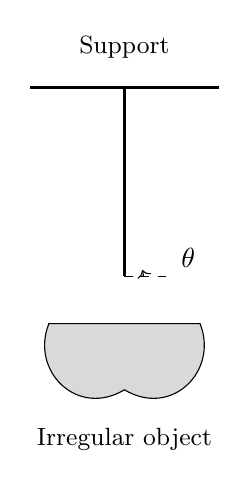
\begin{tikzpicture}[scale=1.2]
  % Support
  \draw[thick] (-1,0) -- (1,0);
  \draw[thick] (-0.3,0) -- (0.3,0);
  % Wire
  \draw[thick] (0,0) -- (0,-2);
  % Object (irregular shape)
  \draw[fill=gray!30] (-0.8,-2.5) .. controls (-1,-3) and (-0.5,-3.5) .. (0,-3.2) .. controls (0.5,-3.5) and (1,-3) .. (0.8,-2.5) -- cycle;
  % Rotation angle
  \draw[dashed] (0,-2) -- (0.5,-2);
  \draw[->] (0.2,-2) arc (0:20:0.2);
  \node[right] at (0.5,-1.8) {$\theta$};
  % Label
  \node[above] at (0,0.2) {\small Support};
  \node[below] at (0,-3.5) {\small Irregular object};
\end{tikzpicture}
\end{center}

\section*{Assistance notes:} LLMs were used as translators and concept explainers. No direct solutions were provided.

\end{document}

